% 18 variables in here:
% h_1 = 10.0, h_2 = 12.0, h_3 = 7.0, h_4 = 15.0, h_5 = 11.0, h_6 = 9.0, ux_1 = 0.0, ux_2 = 0.0, ux_3 = 0.0, ux_4 = 0.0, ux_5 = 0.0, ux_6 = 0.0, uy_1 = 0.0, uy_2 = 0.0, uy_3 = 0.0, uy_4 = 0.0, uy_5 = 0.0, uy_6 = 0.0
\begin{figure}[h!]
\centering
  \quad \subfloat[] {
    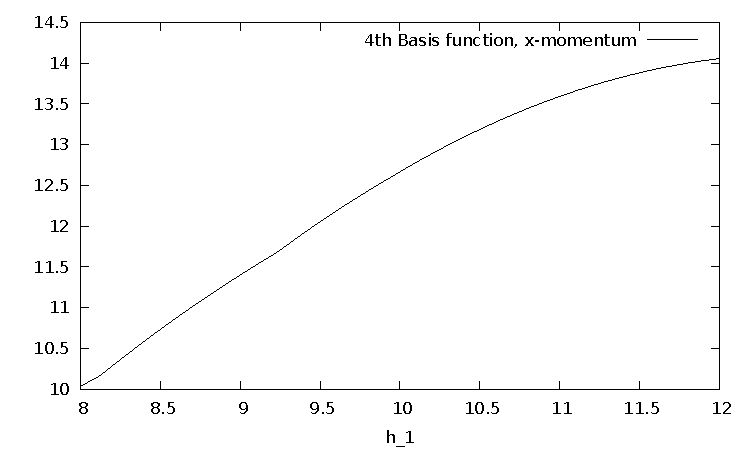
\includegraphics[scale=\zoomfactor]{{{ord2_magnitude_10_nonstd1/y_12.0_7.0_15.0_11.0_9.0_0.0_0.0_0.0_0.0_0.0_0.0_0.0_0.0_0.0_0.0_0.0_0.0f06}}}
  }
  \quad \subfloat[] {
    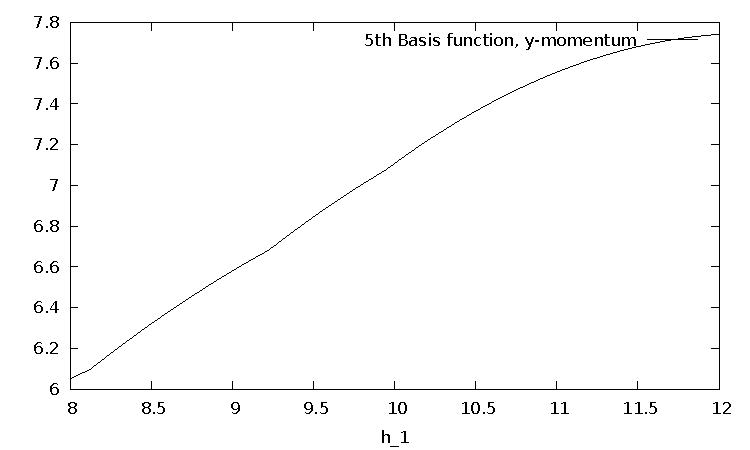
\includegraphics[scale=\zoomfactor]{{{ord2_magnitude_10_nonstd1/y_12.0_7.0_15.0_11.0_9.0_0.0_0.0_0.0_0.0_0.0_0.0_0.0_0.0_0.0_0.0_0.0_0.0f09}}}
  }
\caption{}
\label{fig:ord2_magnitude_10_nonstd1}
\end{figure}

%%% Local Variables:
%%% TeX-master: "../results.tex"
%%% End:
% 18 variables in here:
% h_1 = 10.0, h_2 = 12.0, h_3 = 7.0, h_4 = 15.0, h_5 = 11.0, h_6 = 9.0, ux_1 = 0.0, ux_2 = 0.0, ux_3 = 0.0, ux_4 = 0.0, ux_5 = 0.0, ux_6 = 0.0, uy_1 = 0.0, uy_2 = 0.0, uy_3 = 0.0, uy_4 = 0.0, uy_5 = 0.0, uy_6 = 0.0
\begin{figure}[h!]
\centering
  \quad \subfloat[] {
    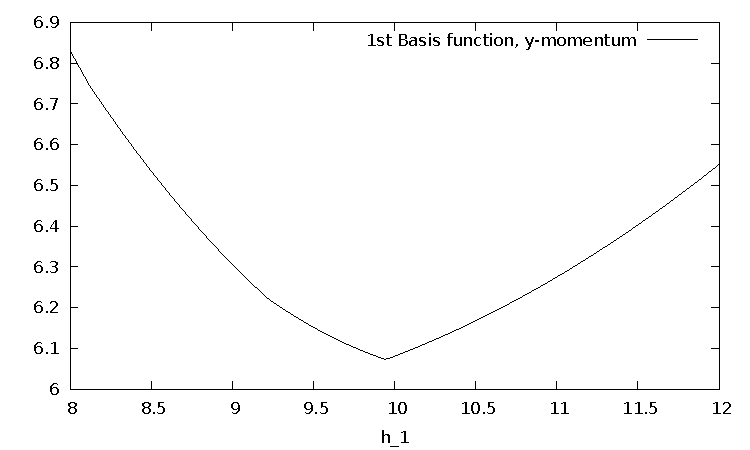
\includegraphics[scale=\zoomfactor]{{{ord2_magnitude_10_nonstd1/y_12.0_7.0_15.0_11.0_9.0_0.0_0.0_0.0_0.0_0.0_0.0_0.0_0.0_0.0_0.0_0.0_0.0f01}}}
  }
  \quad \subfloat[] {
    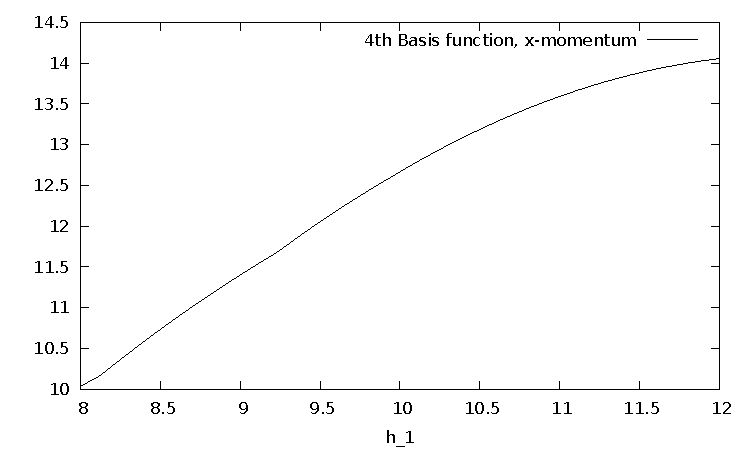
\includegraphics[scale=\zoomfactor]{{{ord2_magnitude_10_nonstd1/y_12.0_7.0_15.0_11.0_9.0_0.0_0.0_0.0_0.0_0.0_0.0_0.0_0.0_0.0_0.0_0.0_0.0f06}}}
  }
  \quad \subfloat[] {
    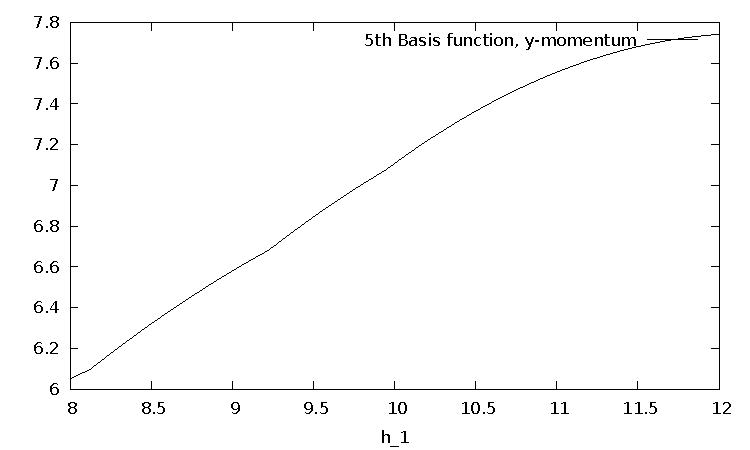
\includegraphics[scale=\zoomfactor]{{{ord2_magnitude_10_nonstd1/y_12.0_7.0_15.0_11.0_9.0_0.0_0.0_0.0_0.0_0.0_0.0_0.0_0.0_0.0_0.0_0.0_0.0f09}}}
  }
\caption{}
\label{fig:ord2_magnitude_10_nonstd1}
\end{figure}

%%% Local Variables:
%%% TeX-master: "../results.tex"
%%% End:
